\documentclass[]{beamer}
\def\short{beamerx}

\usepackage[absolute,overlay]{textpos}

\usepackage{times}
\usepackage{eulervm}

\usepackage{subfig}

\usepackage{graphicx}
\usepackage[normalem]{ulem}
\usepackage{bm}
\usepackage{tikz}

\usepackage{algorithm} %%% added by zhao
\usepackage{algpseudocode} %%% added by zhao

\pgfmathsetseed{\number\pdfrandomseed}
%\usepackage[usenames,dvipsnames]{xcolor}
\newcommand{\N}{\mathcal{N}}

\newcommand{\one}{\overrightarrow{1}}
\newcommand{\R}{\mathbb{R}}
\newcommand{\C}{\mathbb{C}}
\newcommand{\Z}{\mathbb{Z}}
\newcommand{\nnz}{\mathrm{nnz}}
\DeclareMathOperator*{\argmin}{argmin}
\DeclareMathOperator{\diag}{diag}
%\newcommand{\wh}{\widehat}
\newcommand{\wt}{\widetilde}
\newcommand{\ov}{\overline}
%\newcommand{\OPT}{\mathrm{OPT}}
%\newcommand{\poly}{\mathrm{poly}}
\DeclareMathOperator{\rank}{rank}
\DeclareMathOperator{\constraints}{constraints}
\DeclareMathOperator{\variables}{variables}
\DeclareMathOperator{\degree}{degree}
\renewcommand{\i}{\mathbf{i}}
\newtheorem{assumption}[theorem]{Assumption}
\usetikzlibrary{positioning, calc, chains,arrows,patterns,snakes,decorations.pathreplacing}

\definecolor {utorange}   {RGB} {203,96,21}
\definecolor {utblack}    {RGB} {99,102,106}
\definecolor {utbrown}    {RGB} {110,98,89}
\definecolor {utsecbrown} {RGB} {217,200,158}
\definecolor {utsecgreen} {RGB} {208,222,187}
\definecolor {utsecblue}  {RGB} {127,169,174}


\newcommand{\semitransp}[2][35]{\color{fg!#1}#2}
\definecolor{darkgreen}{RGB}{0,100,0}

\definecolor{darkblue}{RGB}{0,0,200}
\definecolor{greyblue}{RGB}{160,160,250}
\definecolor{darkred}{RGB}{180,0,0}
\definecolor{darkpurple}{RGB}{90,0,90}
\newcommand{\W}{{\color{b2}W}} %%%the default color is blue
\newcommand{\B}{{\color{darkgreen}B}}
\definecolor{mygreen}{RGB}{80,180,0}
\newcommand{\A}{{\color{mygreen}A}}
\newcommand{\whA}{{\color{red}\widehat{A}}}
\newcommand{\U}{{\color{red}U}}
\newcommand{\V}{{\color{red}V}}
\newcommand{\T}{{\color{orange}T}}
\renewcommand{\S}{{\color{orange}S}}
\newcommand{\Q}{{\color{darkgreen}Q}}
\renewcommand{\P}{{\color{darkgreen}P}}
\newcommand{\bv}{{\color{b2}b}}
%%%\definecolor{refc} {RGB} {204,102,0}
%%% use orange color for reference
\definecolor{b1}{RGB}{0,102,255}
\definecolor{b2}{RGB}{51,153,255}
\definecolor{b3}{RGB}{153,204,255}
\definecolor{b4}{RGB}{0,51,102}
\definecolor{b5}{RGB}{0,76,153}
\definecolor{b6}{RGB}{0,102,204}
\definecolor{b7}{RGB}{0,128,255}
\definecolor{b8}{RGB}{153,153,255}
\definecolor{b9}{RGB}{51,51,255}

\definecolor{r1}{RGB}{204,0,0}
\definecolor{r2}{RGB}{255,0,0}
\definecolor{r3}{RGB}{255,51,51}
\definecolor{r4}{RGB}{255,102,102}
\definecolor{r5}{RGB}{255,153,153}

\definecolor{g1}{RGB}{0,153,0}
\definecolor{g2}{RGB}{0,204,0}
\definecolor{g3}{RGB}{0,255,0}
\definecolor{g4}{RGB}{51,255,51}
\definecolor{g5}{RGB}{102,255,102}
\definecolor{g6}{RGB}{80,180,0} %%% which is also my green


\definecolor{mycy}{RGB}{204,0,204}
\definecolor{mycy1}{RGB}{255,0,255}
\definecolor{mycy2}{RGB}{255,51,255}
\definecolor{myyellow}{RGB}{153,153,0}

\newcommand{\colone}{{\color{r5}1}}
\newcommand{\coltwo}{{\color{b2}2}}
\newcommand{\colthree}{{\color{mygreen}3}}
\newcommand{\colfour}{{\color{r2}4}}
\newcommand{\colfive}{{\color{b9}5}}
\newcommand{\colsix}{{\color{darkgreen}6}}

\mode<presentation>
{
  % or ...
\defbeamertemplate*{footline}{infolines theme variant}
{
  \leavevmode%
  \hbox{%
  \begin{beamercolorbox}[wd=.25\paperwidth,ht=2.25ex,dp=1ex,center]{author in head/foot}%
%    \usebeamerfont{author in head/foot}\insertshortauthor~~(\insertshortinstitute)
    \usebeamerfont{author in head/foot}\insertshortauthor
  \end{beamercolorbox}%
  \begin{beamercolorbox}[wd=.6\paperwidth,ht=2.25ex,dp=1ex,center]{title in head/foot}%
    \usebeamerfont{title in head/foot}\insertshorttitle
  \end{beamercolorbox}%
  \begin{beamercolorbox}[wd=.15\paperwidth,ht=2.25ex,dp=1ex,right]{date in head/foot}%
    \usebeamerfont{date in head/foot}\insertshortdate{}\hspace*{2em}
    \insertframenumber{} / \inserttotalframenumber\hspace*{2ex} 
  \end{beamercolorbox}}%
  \vskip0pt%
}

\defbeamertemplate*{headline}{split theme 2}
{%
  %\leavevmode%
  \begin{beamercolorbox}[wd=\paperwidth,ht=2.5ex,dp=1.125ex]{section in head/foot}%
    \insertsectionnavigationhorizontal{\paperwidth}{}{\hskip0pt plus1filll}%
  \end{beamercolorbox}%
  \begin{beamercolorbox}[wd=\paperwidth,ht=2.5ex,dp=1.125ex]{subsection in head/foot}%
    \insertsubsectionnavigationhorizontal{\paperwidth}{}{\hskip0pt plus1filll}%
  \end{beamercolorbox}%
}


  %\usetheme{shadow}
  %\setbeamertemplate{headline}[split theme 2]
  \usetheme{Boadilla}
  \setbeamertemplate{footline}[infolines theme variant]
  \setbeamertemplate {navigation symbols} {}

  %\setbeamercolor {normal text} {bg=white, fg=utblack}
  \setbeamercolor {structure} {fg=utorange}
  \setbeamercolor {alerted text} {fg=red!85!black}
  \setbeamercolor {item projected} {use=item,fg=black,bg=item.fg!35}
  \setbeamercolor* {palette primary} {use=structure,fg=white, bg=utorange}
  \setbeamercolor* {palette secondary} {use=structure,bg=utsecbrown}
  \setbeamercolor* {palette tertiary} {use=structure,bg=utsecgreen}
  \setbeamercolor* {palette quaternary} 
  		   {use=structure,fg=structure.fg,bg=utsecblue}
  \setbeamercolor* {framesubtitle} {fg=utbrown}
  \setbeamercolor* {block title} {parent=structure,fg=black,bg=utsecgreen}
  \setbeamercolor* {block body} {fg=black,bg=utblack!10}
  \setbeamercolor* {block title alerted} {parent=alerted text,bg=black!15}
  \setbeamercolor* {block title example} {parent=example text,bg=black!15}

  %\setbeamercovered{transparent}
  % or whatever (possibly just delete it)
}
\newcommand{\wh}{\widehat}
\newcounter{framenumberappendix}
\newcommand{\backupbegin}{
   \setcounter{framenumberappendix}{\value{framenumber}}
}
\newcommand{\backupend}{
   \addtocounter{framenumberappendix}{-\value{framenumber}}
   \addtocounter{framenumber}{\value{framenumberappendix}} 
}

\usepackage[english]{babel}
\usepackage{amsmath}
\usepackage{setspace}
\usepackage{amsthm}
\usepackage{mathrsfs}

\newcommand\hone{\ensuremath{\begin{pmatrix} 1 \\ 1 \\ 1 \\ 1 \end{pmatrix}}}
\newcommand\htwo{\ensuremath{\begin{pmatrix} 1 \\ -1 \\ 1 \\ -1 \end{pmatrix}}}
\newcommand\htwot{\ensuremath{\begin{pmatrix} 1 & -1 & 1 & -1\end{pmatrix}}}
\newcommand\vs{\vspace{3mm}}

\newcommand{\hthree}{\ensuremath{\begin{pmatrix} 1 \\ 1 \\ -1 \\ -1 \end{pmatrix} }}
\newcommand{\hthreet}{\ensuremath{\begin{pmatrix} 1 & 1 & -1 & -1 \end{pmatrix} }}

\newcommand{\hfour}{\ensuremath{\begin{pmatrix} 1 \\ -1 \\ -1 \\ 1 \end{pmatrix} }}
\newcommand{\hfourt}{\ensuremath{\begin{pmatrix} 1 & -1 & -1 & 1 \end{pmatrix} }}


\newcommand{\norm}[2]{\lVert#2\rVert_{#1}}
\newcommand{\abs}[1]{\lvert#1\rvert}
\newcommand{\inner}[1]{\langle#1\rangle}
\DeclareMathOperator{\E}{\mathbb{E}}
\DeclareMathOperator*{\median}{median}
\DeclareMathOperator{\supp}{supp}
\DeclareMathOperator{\poly}{poly}
\DeclareMathOperator{\sign}{sign}
\DeclareMathOperator{\OPT}{OPT}
\def\eps{\epsilon}
\def\R{\mathbb{R}}
\def\X{\mathcal{X}}
\def\C{\mathbb{C}}
\def\F{\mathbb{F}}
\def\Ot{\tilde{O}}
\def\Thetat{\tilde{\Theta}}
\def\Omegat{\tilde{\Omega}}
\def\Err{\mbox{Err}}
\def\Cov{\mbox{Cov}}
\def\Fc{\mathcal{F}}
\newcommand{\SETH}{\mathsf{SETH}}
\renewcommand{\k}{\mathsf{K}}

\subject{Talks}
% This is only inserted into the PDF information catalog. Can be left
% out. 

\newcounter{jumping}

\resetcounteronoverlays{jumping}

\iffalse
%=cf
\fi\iftrue
\makeatletter
\tikzset{
  stop jumping/.style={
    execute at end picture={%
      \stepcounter{jumping}%
      \immediate\write\pgfutil@auxout{%
        \noexpand\jump@setbb{\the\value{jumping}}{\noexpand\pgfpoint{\the\pgf@picminx}{\the\pgf@picminy}}{\noexpand\pgfpoint{\the\pgf@picmaxx}{\the\pgf@picmaxy}}
      },
      \csname jump@\the\value{jumping}@maxbb\endcsname
      \path (\the\pgf@x,\the\pgf@y);
      \csname jump@\the\value{jumping}@minbb\endcsname
      \path (\the\pgf@x,\the\pgf@y);
    },
  }
}
\def\jump@setbb#1#2#3{%
  \@ifundefined{jump@#1@maxbb}{%
    \expandafter\gdef\csname jump@#1@maxbb\endcsname{#3}%
  }{%
    \csname jump@#1@maxbb\endcsname
    \pgf@xa=\pgf@x
    \pgf@ya=\pgf@y
    #3
    \pgfmathsetlength\pgf@x{max(\pgf@x,\pgf@xa)}%
    \pgfmathsetlength\pgf@y{max(\pgf@y,\pgf@ya)}%
    \expandafter\xdef\csname jump@#1@maxbb\endcsname{\noexpand\pgfpoint{\the\pgf@x}{\the\pgf@y}}%
  }
  \@ifundefined{jump@#1@minbb}{%
    \expandafter\gdef\csname jump@#1@minbb\endcsname{#2}%
  }{%
    \csname jump@#1@minbb\endcsname
    \pgf@xa=\pgf@x
    \pgf@ya=\pgf@y
    #2
    \pgfmathsetlength\pgf@x{min(\pgf@x,\pgf@xa)}%
    \pgfmathsetlength\pgf@y{min(\pgf@y,\pgf@ya)}%
    \expandafter\xdef\csname jump@#1@minbb\endcsname{\noexpand\pgfpoint{\the\pgf@x}{\the\pgf@y}}%
  }
}
\makeatother
\else

\includeonlyframes{cf}

\makeatletter
\tikzset{
  stop jumping/.style={}
}
\makeatother
\renewenvironment{textblock}[1]{}{}
\fi

  \tikzset{
    invisible/.style={opacity=0, text=white},
    visible on/.style={alt=#1{}{invisible}},
    alt/.code args={<#1>#2#3}{%
      \alt<#1>{\pgfkeysalso{#2}}{\pgfkeysalso{#3}} % \pgfkeysalso doesn't change the path
    },
    next/.style={visible on=<+->},
  }
\newcommand{\step}{\addtocounter{beamerpauses}{1}}


\makeatletter
\def\beamer@origitem{%
  \@inmatherr\item\@ifnextchar[\@item{\@noitemargtrue\@item[\@itemlabel]%
  \csname beamer@thcfg@item\endcsname% Insert colour in \beamer@thc@fg
  \ifx\beamer@thc@fg\@empty\relax\else\color{\beamer@thc@fg}\fi% Execute colour
  }}
\makeatother
\newcommand{\recolorfg}[1]{\setbeamercolor{normal text}{fg=#1}\setbeamercolor{item}{fg=#1}\color{#1}}

% If you have a file called "university-logo-filename.xxx", where xxx
% is a graphic format that can be processed by latex or pdflatex,
% resp., then you can add a logo as follows:

%\pgfdeclareimage[height=0.5cm]{csail-logo}{csaillogo.png}
%\pgfdeclareimage[height=0.5cm]{mit-logo}{mitlogo.png}
%\logo{\pgfuseimage{mit-logo}\hspace{0.08in}\pgfuseimage{csail-logo}}
\tikzset{
  topright/.style={anchor=north east, xshift=-3mm, yshift=-3mm},
}

\title{Functions that Preserve Manhattan Distance}
\author[Timothy Chu] {Gary Miller, Shyam Narayanan, Mark Sellke}
\institute{~~~~~CMU~~~~~~~~~~~~~~~~~~~~~~~~~MIT
~~~~~~~~~~~~~~~~~~~~~~~~~~~~ Stanford}



% - Use the \inst command only if there are several affiliations.
% - Keep it simple, no one is interested in your street address.

\date{}%2013-04-04}

% Delete this, if you do not want the table of contents to pop up at
% the beginning of each subsection:
\AtBeginSection[]
{
  \begin{frame}<beamer>{Talk Outline}
    \tableofcontents[currentsection]
  \end{frame}
}

% If you wish to uncover everything in a step-wise fashion, uncomment
% the following command: 

%\beamerdefaultoverlayspecification{<+->}



  \tikzset{
    action/.style={draw,rounded corners,fill=cyan,rectangle,align=left},
    filters/.style={fill=pink},
    nopermute/.style = {opacity=0, text opacity=0},
    permute/.style = {},
  }
  \def \innerblock {
    \node (in) {};
    \node[action, permute, right=0cm of in] (permute) {Permute};
        \node[action, filters, right=.5cm of permute] (filters) {Filters};
        \node[right=2.3cm of filters] (center) {$O(k)$};
        \node[right=2.3cm of center] (out) {};
        \node[action, above=.3cm of center] (1sparse1) {1-sparse recovery};
        \node[action, above=.3cm of 1sparse1] (1sparse2) {1-sparse recovery};
        \node[action, below=.3cm of center] (1sparse3) {1-sparse recovery};
        \node[action, below=.3cm of 1sparse3] (1sparse4) {1-sparse recovery};
        \foreach \value in {1,2,3,4}
           \draw[->,thick] (filters) to[out=0,in=180] (1sparse\value.west);
        \foreach \value in {1,2,3,4}
           \draw[-,thick] (1sparse\value.east) to[out=0,in=180] (out);
        \draw[dotted, thick] (center) -- (1sparse1);
        \draw[dotted, thick] (center) -- (1sparse3);
        \draw[->, thick, permute] (permute) -- (filters);
}
\def \outerblock {
  %\node[action, fill=pink, left=0.5cm of filters] (permute) {Permute};
    \node[left=.5cm of weak] (x) {$x$};
    \node[right=.5cm of weak] (xprime) {$\wh{x}'$};
    \draw[->, thick] (out.west) -- (xprime);
    \draw[->, thick, nopermute] (x) -- (filters.west);
    \draw[->, thick, permute] (x) -- (permute.west);
}

  \newenvironment{changemargin}[2]{%
\begin{list}{}{%
\setlength{\topsep}{0pt}%
\setlength{\leftmargin}{#1}%
\setlength{\rightmargin}{#2}%
\setlength{\listparindent}{\parindent}%
\setlength{\itemindent}{\parindent}%
\setlength{\parsep}{\parskip}%
}%
\item[]}{\end{list}}


\begin{document}
\begin{frame}
  \titlepage
  \vspace{-0.4in}
\begin{tikzpicture}
\node<+-> (z) at (-1,1) {{\color{white} . }};
\node<.-> (z) at (10,1) {{\color{white} . }};
\node<.-> (z) at (-1,-1) {{\color{white} . }};
\node<.-> (z) at (10,-1) {{\color{white} . }};
%\node<.-> [] (zz) at ( 4.9,0 ) {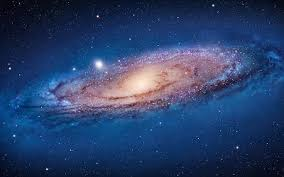
\includegraphics[height=5 cm]{./figs/galaxy}};
%\fill [draw=none, fill=white, fill opacity=0.5] (zz.north west) -- (zz.north east) -- (zz.south east) -- (zz.south west) -- (zz.north west) -- cycle;
    
\node<.-> [] (z) at ( 1.9,0 ) {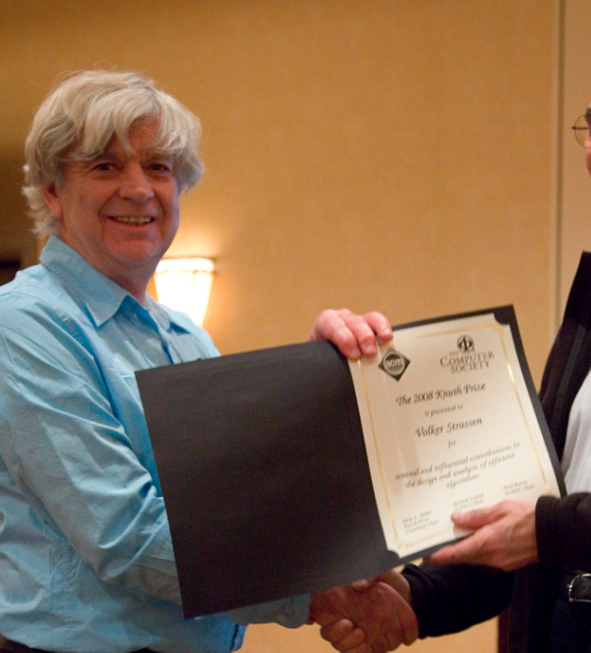
\includegraphics[height=3
  cm]{./figs/gary2}};
\node<.-> [] (z) at ( 4.7,0 ) {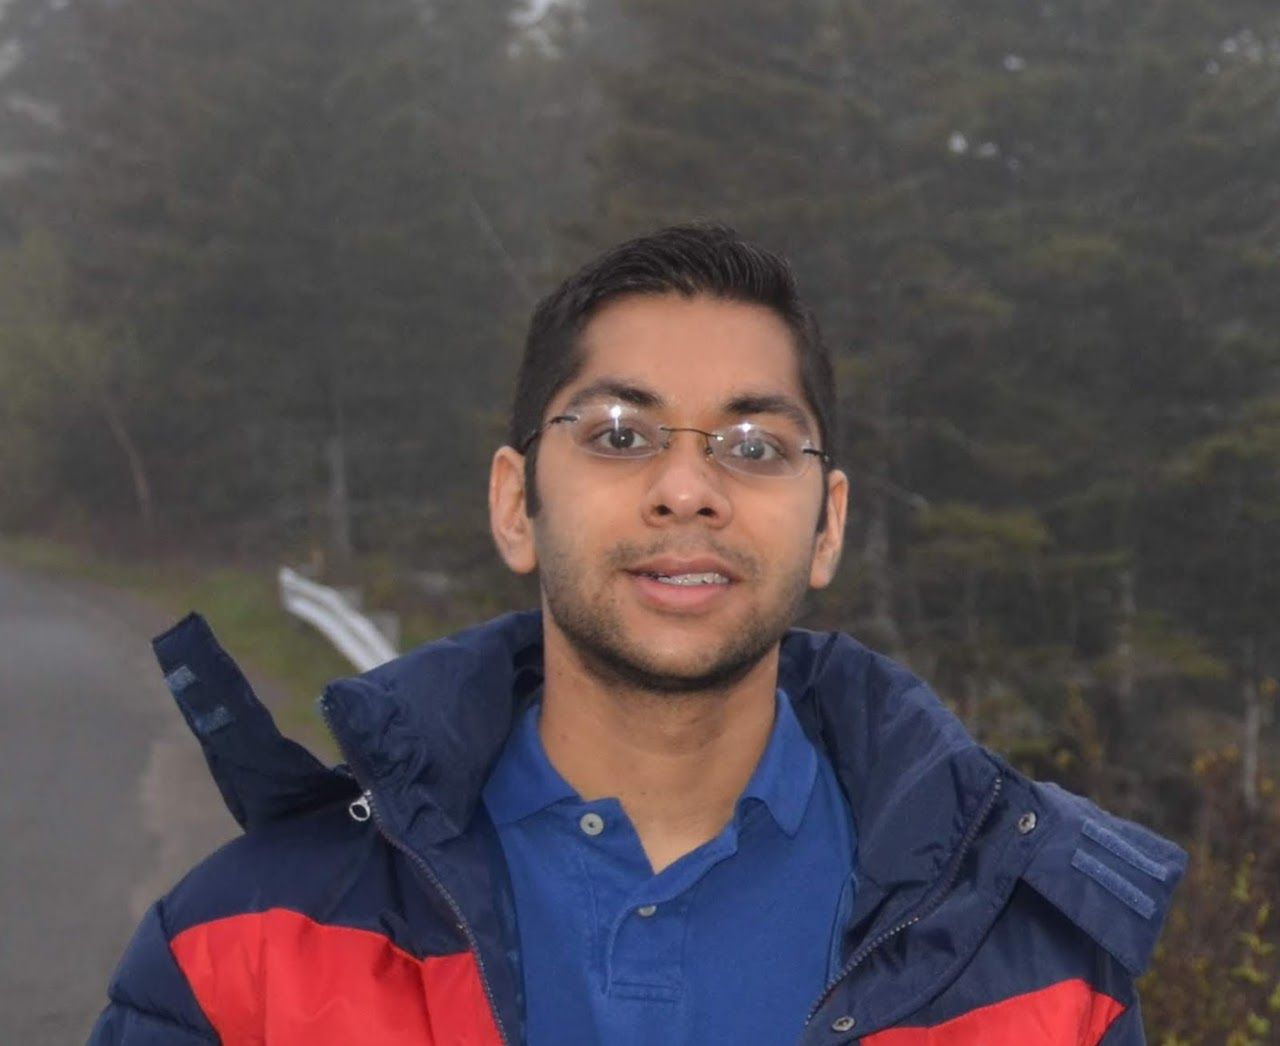
\includegraphics[height=3
  cm]{./figs/shyam}};
\node<.-> [] (z) at ( 7.8,0 ) {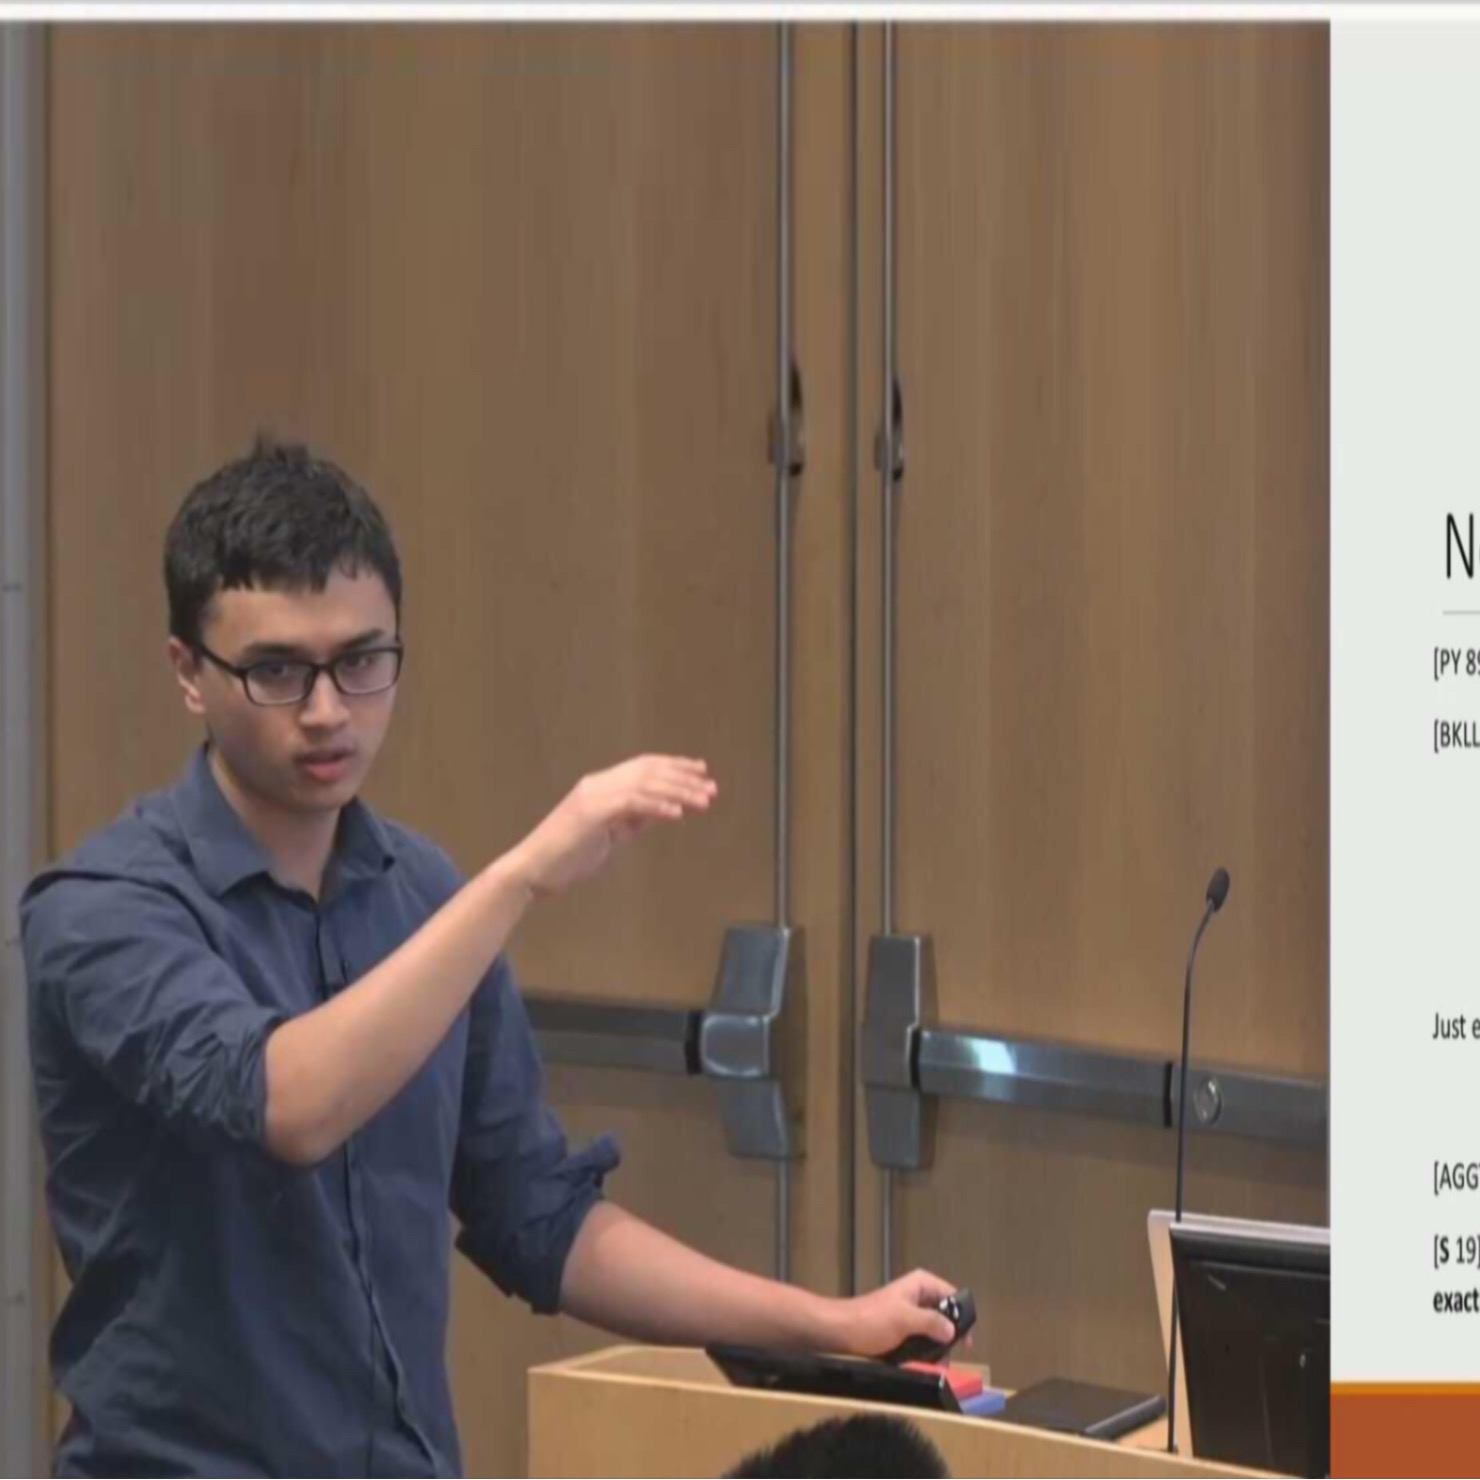
\includegraphics[height=3
  cm]{./figs/marksellke}};
\end{tikzpicture}
      
\end{frame}


\begin{frame}{Manhattan / Taxicab Distance}
   \begin{center}
     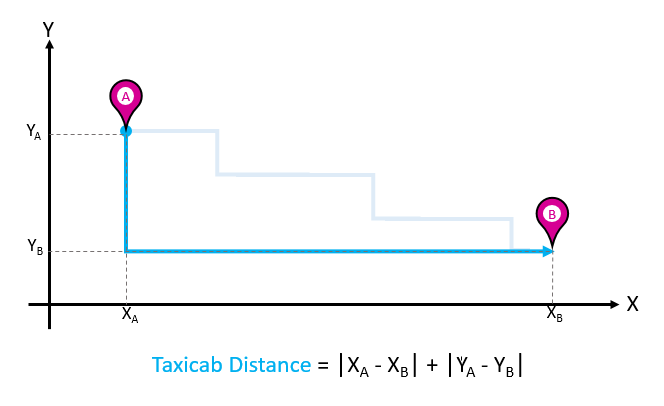
\includegraphics[width=1\textwidth]{figs/taxicab.png}
   \end{center}
\end{frame}

\begin{frame}{A Motivating Puzzle}
  \begin{itemize} 
    \item <+-> Given any $n$ points in any dimension for any $n$,
      compute the $\binom{n}{2}$ Manhattan distances between each pair
      of points. 
      \vs
    \item <+-> Raise each distance to the $2/3$ power.
      \vs
    \item <+-> The result is always a Manhattan distance! 
  \end{itemize}
\end{frame}

\begin{frame} {Why?}
   \begin{center}
     
\includegraphics[width=1\textwidth]{figs/why.jpg}
   \end{center}
\end{frame}
\begin{frame}{A Simple Example}
  \begin{itemize}
    \item <+-> Given $3$ points on a line at at $0, 1$ and $2$, compute
      Manhattan distances between each pair of points.
      \vs
    \item <+-> Raise each distance to the $2/3$ power.
      \vs
    \item <+-> Find $3$ points whose Manhattan distances match these
      powered distances!
  \end{itemize}
\end{frame}

\begin{frame}{A Simple Example}
  \begin{itemize}
    \item <+-> Pairwise distances: $1, 1, 2$.
      \vs
    \item <+-> Powered distances: $1, 1, 2^{2/3}$.
      \vs
    \item <+-> \begin{align}
      & a = \left(\frac{1}{2} + \frac{2^{2/3}}{4}\:,\enspace
      \frac{1}{2}-\frac{2^{2/3}}{4}\right)\nonumber \\
      & b = (0, 0) \nonumber \\
      & c=\left(\frac{1}{2}-\frac{2^{2/3}}{4}\:,\enspace
      \frac{1}{2}+\frac{2^{2/3}}{4}\right). \nonumber
    \end{align}
  \end{itemize}
\end{frame}

\begin{frame}
    \textbf{Definition:} The function $f(x) = x^{2/3}$ \textbf{sends}
  Manhattan distances to Manhattan distances.
\end{frame}

\begin{frame}{The Core Mystery of our Talk}
  \begin{itemize} 
    \item <+-> 
      Why does $x^{2/3}$ send Manhattan distances to
      Manhattan distances?
  \end{itemize}
%  \pause
%   \begin{center}
%     
\includegraphics[width=0.3\textwidth]{figs/mysterybox.jpg}
%   \end{center}

\end{frame}



\begin{frame}{Our Work}
  \begin{itemize}[<+->]
  \item \textbf{Our work}: A self-contained, `simpler' proof that Bernstein
  functions send Manhattan distances to Manhattan distances.
      \vs
  \begin{itemize}[<+->]
    \item This was known before, with a more intricate proof
      [Schoenberg '37 + Assouad '80]
      \vs
  \end{itemize}
\item \textbf{Our Work:} Only Benstein Manhattan distances to Manhattan
    distances.
      \vs
  \begin{itemize}[<+->]
    \item This is new.
  \end{itemize}
      \vs
\item Our talk focuses on the first point.
  \end{itemize}
\end{frame}


\begin{frame}{Takeaways for the Talk}
  \begin{itemize}[<+->]
  \item Why does $x^{2/3}$ send Manhattan distances to Manhattan
  distances? A full proof.
  \item A deeper understanding of background tools:
  \begin{enumerate} [<+->]
  \item Manhattan distances
  \item How to determine whether a distance embeds into (squared)
  \textbf{Euclidean} distance.
  \item \textbf{Bonus}: A hidden use of Representation Theory of the
  group $\mathbb{Z}_2^n$.

  \end{enumerate}
  \end{itemize}
\end{frame}


%\begin{frame}{Proof Outline}
  \begin{itemize}[<+->]
  \item (Known) Any Manhattan distance can be realized as a Manhattan
  distance between a subset of corners of a high dimensional rectangle (hyperbox).
  \item (New) Any Bernstein function, when applied to a Manhattan
  distance, gives a \textbf{squared} Euclidean distance.
  \item This embedding into squared Euclidean distance happens to map
  vertices to corners of a hyperbox. Thus, these distances are secretly
  Manhattan distances.
  \item Therefore, Any Bernstein function, when applied to a Manhattan
  distance, gives a Manhattan distance.
  \end{itemize}
\end{frame}

% \begin{frame}{Background Roadmap}
  \begin{enumerate} 
  \item {\color{blue}Bernstein functions}
  \item Manhattan distances
  \item How to determine whether a distance embeds into (squared)
  \textbf{Euclidean} distance.
  \item \textbf{Bonus}: A hidden use of Representation Theory of the
  group $\mathbb{Z}_2^n$.

  \end{enumerate}
\end{frame}


% \begin{frame}{Bernstein Functions}
\textbf{Theorem:} A function sends Manhattan distances to Manhattan
distances if and only if it is \textbf{Bernstein.}
\vs

\pause

  A \textbf{Bernstein function} is a (positive valued) function with
  positive derivative, negative second derivative, positive third derivative,
  negative fourth derivative$\ldots$ on $x \geq 0$.
\end{frame}

\begin{frame}{Bernstein Functions Examples}
Examples of Bernstein Functions:
\pause
  \begin{itemize}[<+->]
    \item $f(x) = x^s$ for any $0 \leq s \leq 1$.
    \item $f(x) = 1-e^{-tx}$ for any $ t > 0$.
    \item $f(x) = 1 - \frac{1}{1+x}$.
    \item $f(x) = \log(1+x)$.
    \item Any positive linear combination of the above.
  \end{itemize}
\end{frame}

% \begin{frame}{Where else are Bernstein functions useful?}
% Besides for metric transform results (such as ours, and Schoenberg's),
%         Bernstein functions appear in:
%   \begin{itemize}[<+->]
%   \item Probability theory (Laplace Transforms),
%   \item Machine Learning (Kernel methods [Smola '96]),
%   \item Sphere packing [Cohn '02],
%   \item Harmonic Analysis (Reproducing Kernel Hilbert Spaces),
%   \end{itemize}
%   \pause
%   and more.
% \end{frame}

\begin{frame}{Background Roadmap}
  \begin{enumerate} 
  \item {\color{blue}Manhattan distances}
  \item How to determine whether a distance embeds into (squared)
  \textbf{Euclidean} distance.
  \item \textbf{Bonus}: A hidden use of group Representation Theory.
  \end{enumerate}
\end{frame}


\begin{frame}{Manhattan / Taxicab Distance}
   \begin{center}
     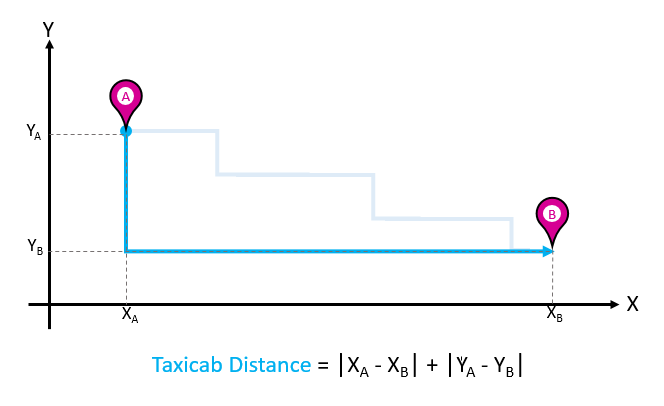
\includegraphics[width=1\textwidth]{figs/taxicab.png}
   \end{center}
\end{frame}

% \begin{frame}{Some simple puzzles on Manhattan Distance}
%   \begin{itemize}[<+->]
%   \item Can the Euclidean distance between two points exceed the
%   Manhattan distance?
%   \end{itemize}
%   \pause
%   \begin{center}
%      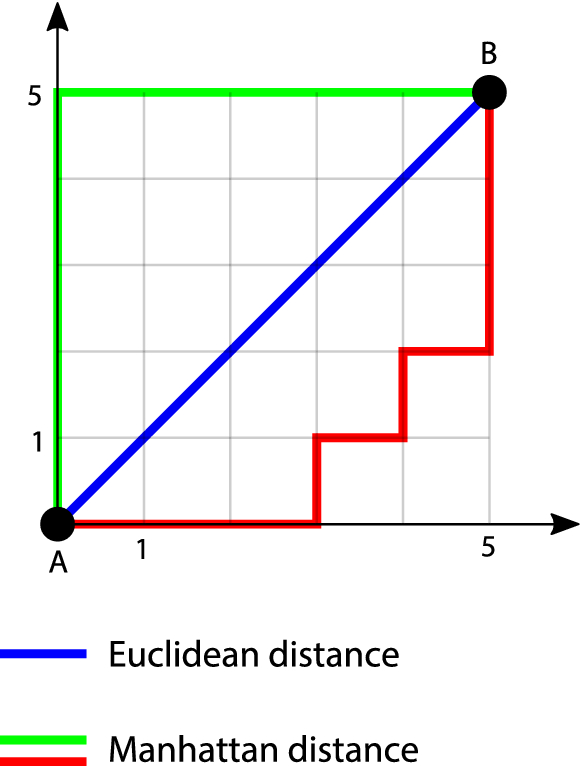
\includegraphics[width=0.4\textwidth]{figs/euclidean_vs_manhattan}
%   \end{center}
% \end{frame}


\begin{frame}{Puzzles on Manhattan distance}
  \begin{itemize}[<+->]
%  \item {\color{darkgreen} Show that any three point metric is a
%    Manhattan distance [Easy]}
%  \item {\color{orange} Is every metric a Manhattan distance? [Medium]}
  \item Show that any three point Manhattan metric is
    equivalent to a Manhattan metric on three corners of some high
      dimensional hyperbox.
  \end{itemize}
\end{frame}

% \begin{frame}{Is every metric a Manhattan distance?}
% No.
% \pause
%    \begin{center}
%      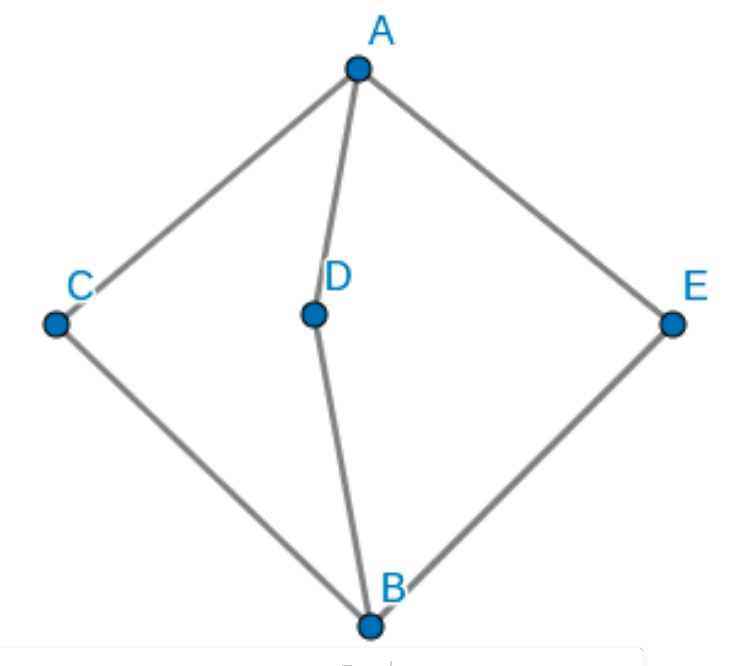
\includegraphics[width=0.5\textwidth]{figs/manhattan_counterexample}
%    \end{center}
%  \end{frame}


\begin{frame}{Are Manhattan distances equivalent to Manhattan distances
on a hyperbox?}
\only<1-3>

\only<1>{
   \begin{center}
     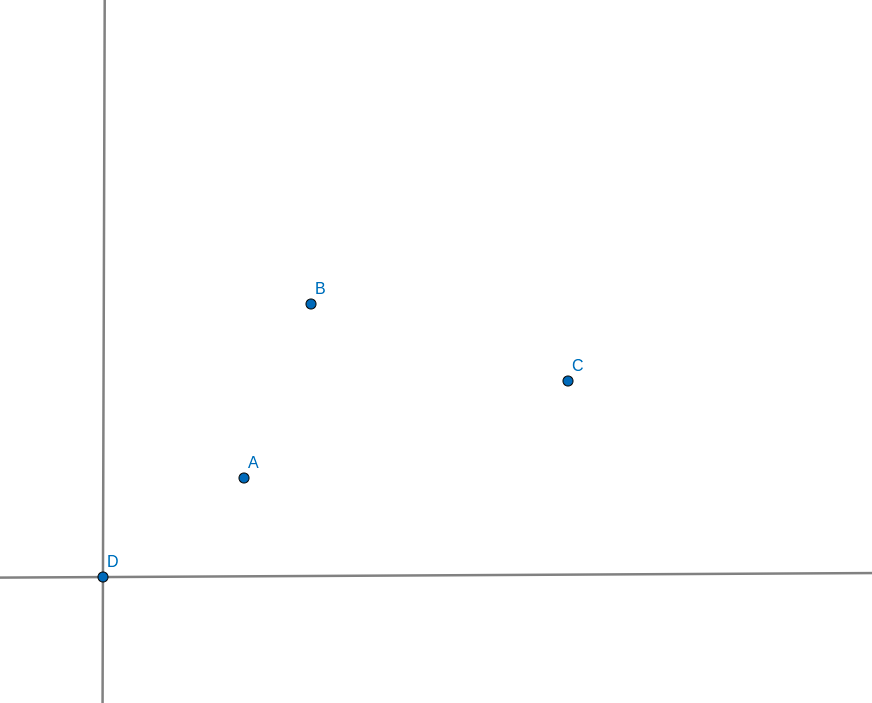
\includegraphics[width=0.6\textwidth]{figs/boxtheorem1.png}
   \end{center}
}
\only<2>{
   \begin{center}
     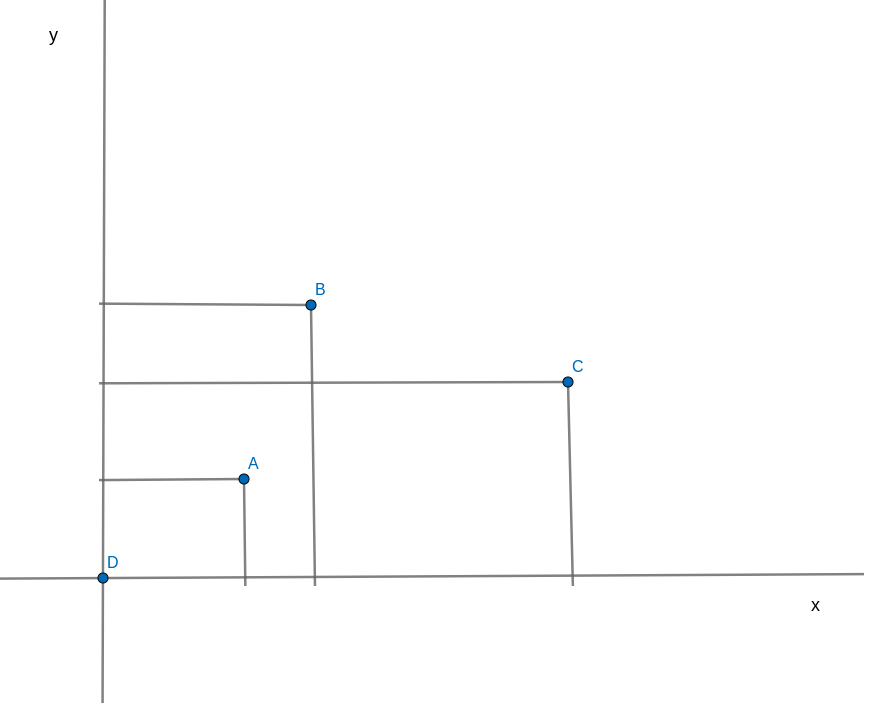
\includegraphics[width=0.6\textwidth]{figs/boxtheorem2.png}
   \end{center}
}
\only<3>{
   \begin{center}
     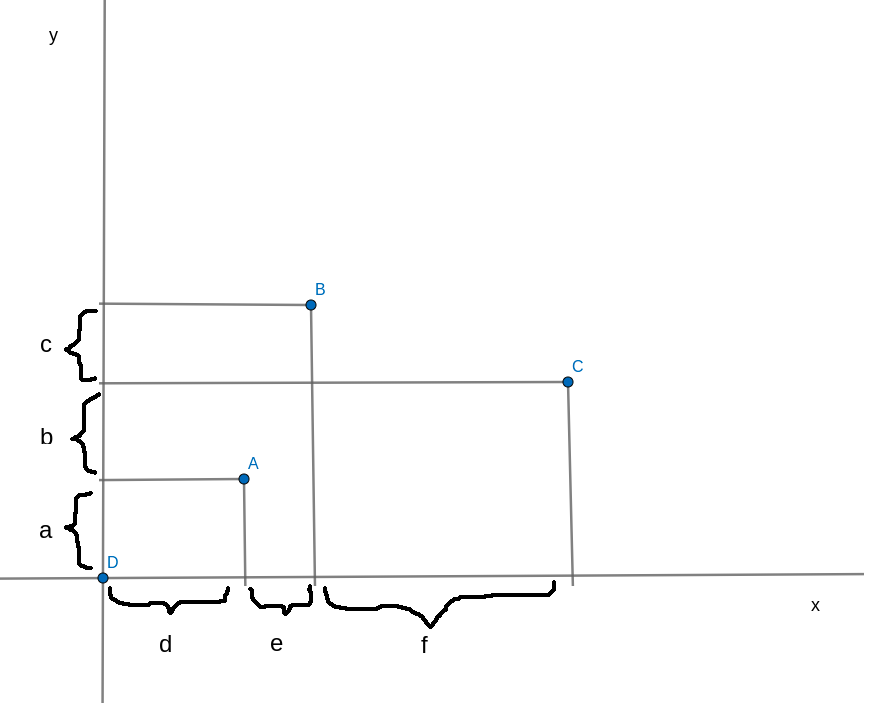
\includegraphics[width=0.6\textwidth]{figs/boxtheorem2-05.png}
   \end{center}
}
\end{frame}
\begin{frame}{Are Manhattan distances equivalent to Manhattan distances
  on a hyperbox?}
   \begin{center}
     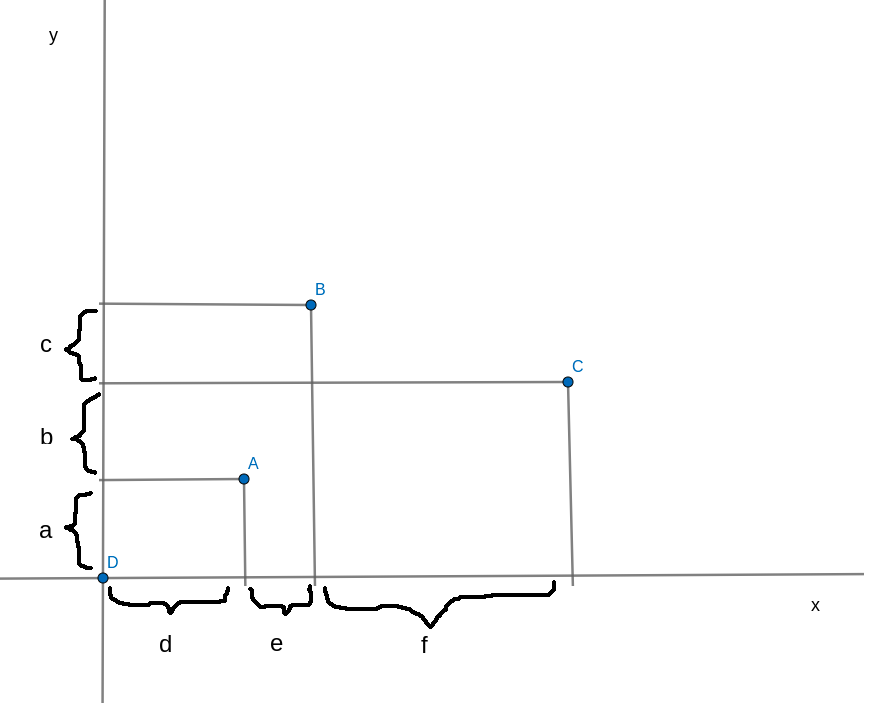
\includegraphics[width=0.6\textwidth]{figs/boxtheorem2-05.png}
   \end{center}
\begin{itemize}[<+->]
 \item Let $A'$ be the point $(a, 0, 0, d, 0, 0)$.
 \item Let $B'$ be the point $(a, b, c, d, e, 0)$.
 \item Let $C'$ be the point $(a, b, 0, d, e, f)$.
\end{itemize}
% \only<4>{
%    \begin{center}
%      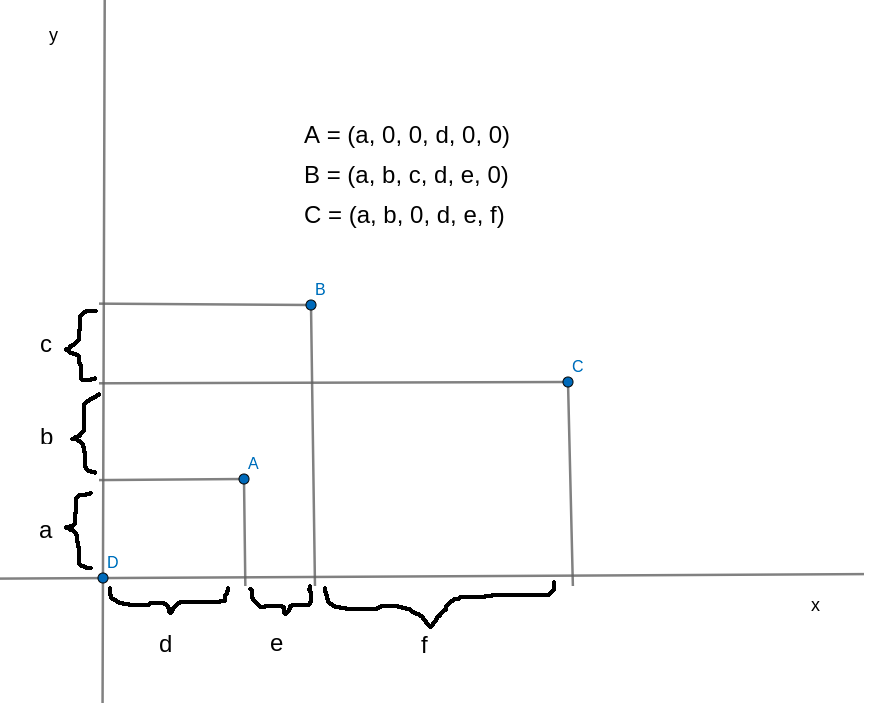
\includegraphics[width=0.6\textwidth]{figs/boxtheorem3.png}
%    \end{center}
% }

\end{frame}

\begin{frame}{Background Roadmap}
  \begin{enumerate} 
  \item Manhattan distances
  \item {\color{blue}How to determine whether a distance embeds into (squared)
    \textbf{Euclidean} distance.}
  \item \textbf{Bonus}: A hidden use of group Representation Theory.
  \end{enumerate}
\end{frame}


% \begin{frame}{What is a criterion for when points embed into
%   Euclidean Distance?} 
%   \begin{itemize}[<+->]
%   \item  A distance $d$ on an $n$ point set is a Euclidean distance if and only
%   if the matrix $D$ with:
% 
%  \[ D_{ij} = d(i, j)^2 \]
% 
%  has the property that $x^T D x \leq 0$ for all $x \bot 1$.
%   \end{itemize}
% \end{frame}

\begin{frame}{What is a criterion for when points embed into
  \textbf{Squared}
  Euclidean Distance?} 
  \begin{itemize}[<+->]
  \item  A distance $d$ on a set $\{x_1, \ldots x_n\}$ is a \textbf{squared} Euclidean distance if and only
  if the matrix $D$ with:

 \[ D_{ij} = d(x_i, x_j) \]
 \pause
 has the property that $x^T D x \leq 0$ for all $x \bot 1$ [Schoenberg
 '35].
 \pause
 \item A matrix with this property is called a \textbf{negative type}
 matrix. (Classical)
  \item Here, we assume $d(x,x) = 0$ and $d(x,y) = d(y,x)$. We do not
  assume metric property.
  \item But how can we test for this???
  \end{itemize}
\end{frame}
% \begin{frame}{Example} 
%   \begin{itemize}[<+->]
%   \item Consider a 2 point set $\{x, y\}$ where $d(x,y) = \pi$.
%   \item 
%   $ \begin{pmatrix} 
%   0 & \pi \\
%   \pi & 0
%   \end{pmatrix}
%   $
%   has the property that $x^T D x  \leq 0$ for $x \perp \overrightarrow{1}$.
%   \item Therefore, $d$ is a squared Euclidean distance.
%   \end{itemize}
% \end{frame}
% \begin{frame}{Example} 
%   \begin{itemize}[<+->]
%   \item Consider the 3 points $(0, 0), (0, 1), (1, 1)$.
%   \item The Euclidean distances are $1, 1, \sqrt{2}$.
%   \item The squared Euclidean distances are $1, 1, 2$.
%   \item Therefore (by our theorem):
%     \pause
%      \[D = 
%   \begin{pmatrix} 
%   0 & 1 & 2 \\
%   1 & 0 & 1 \\
%   2 & 1 & 0
%   \end{pmatrix}
%   \]
%   \pause
%   has the property that $x^T D x  \leq 0$ for $x \perp \overrightarrow{1}$.
%   \end{itemize}
% \end{frame}


\begin{frame}{A Sufficient Criterion for Negative Type Matrices}
  \begin{itemize}[<+->]
  \item Let $D$ be a symmetric matrix.
  \item Suppose $D$ has eigenvector $\overrightarrow{1}$, and all other
  eigenvectors have negative eigenvalue.
  \item Show that $D$ is negative type: $x^T D x \leq 0$
      for all $x \perp 1$.
  \end{itemize}
\end{frame}

 \begin{frame}{Example} 
   \begin{itemize}[<+->]
   \item Let 
   $ D = \begin{pmatrix} 
   0 & 1 \\
   1 & 0
   \end{pmatrix}.$
   This has eigenvector $\overrightarrow{1}$, and all other eigenvectors $(1,
       -1)$ have negative eigenvalue.
   \item Therefore, it of negative type, and the associated distance is
   a squared Euclidean distance.
   \end{itemize}
 \end{frame}

 \begin{frame}{Exercise} 
   \begin{itemize}[<+->]
   \item Show that
   $ D = \begin{pmatrix} 
   0 & 1 & 1\\
   1 & 0 & 1\\
   1 & 1 & 0\\
   \end{pmatrix}.$
   is a negative type matrix!
   \end{itemize}
 \end{frame}
\begin{frame}{A Sufficient Criterion for Showing a Distance is Squared
  Euclidean}

Let $d$ be a distance on set $x_1, \ldots x_n$, such that the matrix
$D$ with $D_{ij} = d(x_i, x_j)$ satisfies:
  \begin{itemize}
  \item $D$ has $\one$ as an eigenvector.
  \item  All other eigenvalues of $D$ are negative.
  \end{itemize}
  Then $D_{ij}$ embeds into squared Euclidean distance!
\end{frame}



%\begin{frame}{}
%  \begin{itemize}[<+->]
%  \item Why does $x^{2/3}$ send Manhattan distances to squared Euclidean
%  distances?
%  \item Recall that any Manhattan distance can be realized as a
%  Manhattan distance on some corners of some hyperbox.
%  \item Thus: we will prove $x^{2/3}$ sends Manhattan distances on
%  hyperboxes, to squared Euclidean distance.
%  \end{itemize}
%\end{frame}
%
%\begin{frame}{}
%  \begin{itemize}[<+->]
%  \item Let's do it for the $2$ dimensional hyperbox, aka the rectangle.
%  \end{itemize}
%\end{frame}

\begin{frame}{$x^{2/3}$ sends Manhattan distances to Manhattan
  distances}
  \begin{itemize}[<+->]
  \item Without loss of generality, let's assume the Manhattan distances
  are the full set of corners on some hyperbox.
  \item We will show that $x^{2/3}$ sends these distances to squared
  Euclidean distances \textbf{on a hyperbox}. 
  \item Squared Euclidean distances on a hyperbox are Manhattan
  distances!
  \end{itemize}
\end{frame}

\begin{frame}{$x^{2/3}$ sends Manhattan distances to squared Euclidean
  distances}
  \begin{itemize}[<+->]
  \item We show $x^{2/3}$ sends Manhattan distances on a box to squared
  Euclidean distance.
  \item We do `proof by example', using a $2$ dimensional box.
  \end{itemize}
\end{frame}

\begin{frame}{$x^{2/3}$ sends Manhattan-on-a-box to Squared Euclidean}
  \begin{itemize}[<+->]
  \item Consider a rectangle with side lengths $a, b$. Let $f(x) =
  x^{2/3}$.
  \item Let $x_1 = (0, 0), x_2 = (a, 0), x_3 = (b, 0), x_4 = (a, b)$.
  \item The matrix $D$ with $D_{ij} = d(x_i, x_j)$ is:
  \[ \begin{pmatrix}
  0 & f(a) & f(b) & f(a+b)\\
  f(a) & 0 & f(a+b) & f(b)\\
  f(b) & f(a+b) & 0 & f(a)\\
  f(a+b) & f(b) & f(a) & 0
  \end{pmatrix}
  \]
  \item Claim: $\one$ is an eigenvector of $D$. (Why?)
  \item Claim: All other eigenvalues of $D$ are negative or $0$. (Why?)
%  \item Therefore: $D$ is negative type! 
  \item Therefore: our Manhattan distances raised to the $2/3$ power are
  squared Euclidean distances.
  \end{itemize}
\end{frame}

\begin{frame}{$x^{2/3}$ sends Manhattan-on-a-box to Squared Euclidean}
  \[ D = \begin{pmatrix}
  0 & f(a) & f(b) & f(a+b)\\
  f(a) & 0 & f(a+b) & f(b)\\
  f(b) & f(a+b) & 0 & f(a)\\
  f(a+b) & f(b) & f(a) & 0
  \end{pmatrix}
  \]
  $f(x)=x^{2/3}$
  \begin{itemize}[<+->]
  \item Claim: $\one$ is an eigenvector of $D$ with eigenvalue $0 +
  f(a)+f(b)+f(a+b)$
  \item Claim: The other eigenvectors of $D$ are the columns of the $2$ by
  $2$ Hadamard matrix:
  \[ \begin{pmatrix}
  1 & 1 & 1 & 1 \\
  1 & -1 & 1 & -1 \\
  1 & 1 & -1 & -1 \\
  1 & -1 & -1 & 1 \\
  \end{pmatrix}
  \]
  \item Why? You can verify this by calculation. 
  \item This is the secret use of representation theory: boxes are
  symmetric under axial reflection, and for any permutation matrix $M$
  corresponding to permuting the corners of our box, $DM = MD$. 
  \item Any matrix with this property has Hadamard eigenvectors.
  \end{itemize}
\end{frame}

\begin{frame}{$x^{2/3}$ sends Manhattan-on-a-box to Squared Euclidean}
  \[ D = \begin{pmatrix}
  0 & f(a) & f(b) & f(a+b)\\
  f(a) & 0 & f(a+b) & f(b)\\
  f(b) & f(a+b) & 0 & f(a)\\
  f(a+b) & f(b) & f(a) & 0
  \end{pmatrix}
  \]
  $f(x)=x^{2/3}$
  \begin{itemize}[<+->]
  \item We are knee deep in showing $D$ is of negative type. $x^T D x
  \leq 0$ for all $x \perp \one$.
  \item We are showing $D$ has $\one$ as an eigenvector, and all other
  eigenvectors are columns of the $2$ by $2$ Hadamard matrix 
  $ \begin{pmatrix}
  1 & 1 & 1 & 1 \\
  1 & -1 & 1 & -1 \\
  1 & 1 & -1 & -1 \\
  1 & -1 & -1 & 1 \\
  \end{pmatrix}
 $. 
 \item
  The associated eigenvalues, we claim, are negative. We will show this
  by direct computation.
  \end{itemize}
\end{frame}

\begin{frame}{$x^{2/3}$ sends Manhattan-on-a-box to Squared Euclidean}
  \[ D = \begin{pmatrix}
  0 & f(a) & f(b) & f(a+b)\\
  f(a) & 0 & f(a+b) & f(b)\\
  f(b) & f(a+b) & 0 & f(a)\\
  f(a+b) & f(b) & f(a) & 0
  \end{pmatrix}
  \]
  \begin{itemize}[<+->]
  \item The eigenvalue $\lambda$ corresponding to eigenvector $v = (1, -1, 1, -1)$
  satisfies
  $D 
  \begin{pmatrix}
  1 \\
  -1\\
  1 \\
  -1\\
  \end{pmatrix} 
  = \lambda 
  \begin{pmatrix}
  1 \\
  -1\\
  1 \\
  -1\\
  \end{pmatrix} 
  $.
  \item This can be computed by evaluating $D_1v$ where $D_1$ is the
  first row of $D$.
  \item This is $-f(a) + f(b) -f(a+b)$.
  \item $= -\int_0^a f'(x)dx  -\int_b^{a+b} f'(x)dx$
  \item Why is this eigenvalue negative, when $f = x^{2/3}$?
  \end{itemize}
\end{frame}

%  \begin{frame}{$x^{2/3}$ sends Manhattan-on-a-box to Squared Euclidean}
%    \[ D = \begin{pmatrix}
%    0 & f(a) & f(b) & f(a+b)\\
%    f(a) & 0 & f(a+b) & f(b)\\
%    f(b) & f(a+b) & 0 & f(a)\\
%    f(a+b) & f(b) & f(a) & 0
%    \end{pmatrix}
%    \]
%    \begin{itemize}[<+->]
%    \item Likewise, the eigenvector corresponding to 
%    $v = \begin{pmatrix}
%    1 \\
%    1\\
%    -1 \\
%    -1\\
%    \end{pmatrix}$
%    is $D_1 v$, which equals $f(a) - f(b) -f(a+b)$
%    \item $= -\int_0^b f'(x)dx  + -\int_a^{a+b} f'(x)dx$
%    \item Why is this eigenvalue negative?
%    \end{itemize}
%  \end{frame}
 
 \begin{frame}{$x^{2/3}$ sends Manhattan-on-a-box to Squared Euclidean}
   \[ D = \begin{pmatrix}
   0 & f(a) & f(b) & f(a+b)\\
   f(a) & 0 & f(a+b) & f(b)\\
   f(b) & f(a+b) & 0 & f(a)\\
   f(a+b) & f(b) & f(a) & 0
   \end{pmatrix}
   \]
   \begin{itemize}[<+->]
   \item The eigenvalue of $D$ corresponding to $
   v = \begin{pmatrix} 1 \\
   -1\\
   -1 \\
   1\\
   \end{pmatrix}$
   equals
   $D_1v = f(a) + f(b) -f(a+b)$
   \item $= \int_0^a \int_0^b f''(x+y) dx dy$
   \item Why is this eigenvalue negative?
   \end{itemize}
 \end{frame}
 
 \begin{frame}{$x^{2/3}$ sends Manhattan-on-a-box to Squared Euclidean}
   \begin{itemize}[<+->]
   \item We showed that our matrix $D$ has eigenvector $\one$ and all
   other eigenvalues negative. This means it is negative type.
   \item $D$ being negative type is equivalent to the distance being a
   squared Euclidean distance. (Presented earlier without proof).
   \item Thus, $x^{2/3}$ sends Manhattan distance to squared Euclidean
   distance.
   \item What property of $x^{2/3}$ did we use? What is the general
   property of functions $f$?
   \end{itemize}
 \end{frame}
 
 \begin{frame}{$x^{2/3}$ sends Manhattan-on-a-box to Manhattan}
   \begin{itemize}[<+->]
   \item We showed a weaker result than the one we wanted: $x^{2/3}$
   sends Manhattan-on-a-box to squared Euclidean.
   \item But I promised you that $x^{2/3}$ would send Manhattan-on-a-box
   to squared-Euclidean-on-a-box.
   \item We show this by backing out the actual embedding.
   \end{itemize}
 \end{frame}
 
 \begin{frame}{Given a squared Euclidean distance, how do I find the
   embedding?}
   \begin{itemize}[<+->]
   \item Let's say you have your squared Euclidean distance in a matrix
   $D$.
   \item You can find the matrix of dot products by computing: 
   $ M = -\Pi D \Pi / 2$ where $\Pi$ is the projection matrix off the all
   ones vector (Well known, exercise for the reader).
   \item Any matrix $P$ with $PP^T = M$, has row vectors which realize
   the squared Euclidean distance $D$. (Well known, exercise for the
       reader).
   \end{itemize}
 \end{frame}
 

\begin{frame}{Why does $M = -\Pi D \Pi/2$ give a matrix of
  mean-centered
  products?}
  \begin{itemize}[<+->]
   \item Let
   $J$ be the all ones matrix.
   \item Let $P$ be the matrix whose $i^{th}$ row is $p_i$.
   \item Let $p_i$ be points such that \\ $D_{ij} = \|p_i -
   p_j\|_2^2 = |p_i|_2^2 + |p_j|_2^2 - 2\langle p_i, p_j \rangle $.  
     \pause
   \[
   D = 
%   \begin{pmatrix} |p_1|_2^2 & |p_1|_2^2 & \ldots & |p_1|_2^2 \\
%     |p_2|_2^2 & |p_2|_2^2 & \ldots & |p_2|_2^2 \\
%     \ldots \\
%     |p_n|_2^2 & |p_n|_2^2 & \ldots & |p_n|_2^2 
%   \end{pmatrix} 
%   +
%   \begin{pmatrix} |p_1|_2^2 & |p_2|_2^2 & \ldots & |p_n|_2^2 \\
%     |p_1|_2^2 & |p_2|_2^2 & \ldots & |p_n|_2^2 \\
%     \ldots \\
%     |p_1|_2^2 & |p_2|_2^2 & \ldots & |p_n|_2^2 
%   \end{pmatrix} 
   \begin{pmatrix} |p_1|^2 & 0 & 0 & \ldots \\
     0 & |p_2|^2 & 0 &  \ldots \\
     \ldots \\
     0 & 0 & \ldots & |p_n|^2
     \end{pmatrix}  J
     + J 
   \begin{pmatrix} |p_1|^2 & 0 & 0 & \ldots \\
     0 & |p_2|^2 & 0 &  \ldots \\
     \ldots \\
     0 & 0 & \ldots & |p_n|^2
     \end{pmatrix}
       \]
       \[
     - 2PP^T
     \]
     \pause

     \item Recall that we defined $M = -\Pi D \Pi/2$ where $\Pi$
     projects off the all ones vector.
     \item Then $M = \Pi PP^T \Pi$ \pause $= PP^T$.
  \end{itemize}
\end{frame}

 \begin{frame}{Given a squared Euclidean distance, how do I find the
   embedding?}
   \begin{itemize}
   \item Let's say you have your squared Euclidean distance in a matrix
   $D$.
   \item You can find the matrix of dot products by computing: 
   $ M = -\Pi D \Pi / 2$ where $\Pi$ is the projection matrix off the all
   ones vector (Well known, exercise for the reader).
   \item Any matrix $P$ with $PP^T = M$, has row vectors which realize
   the squared Euclidean distance $D$. (Well known, exercise for the
       reader).
   \end{itemize}
 \end{frame}

 \begin{frame}{Given a squared Euclidean distance, how do I find the
   embedding?}
   \begin{itemize}[<+->]
   \item Let's try this on our matrix $D$ on a $2$ dimensional box, after
   applying $x^{2/3}$ to the distances. The eigenvectors of $D$ are $h_1 = \hone, h_2 = \htwo,
   h_3 = \hthree, h_4 = \hfour.$
   \item We know $D = \lambda_1 h_1 h_1^T  + \lambda_2 h_2 h_2^T +
   \lambda_3 h_3 h_3^T + \lambda_4 h_4 h_4^T$.
   \item Here, $\lambda_i$ is the eigenvalue corresponding to
   eigenvector $h_i$.
   \item Then $M$, the matrix of dot products, equals $- \Pi D \Pi / 2$ where $\Pi$ is the projection matrix
   off $\one$.
   \item $M = \frac{1}{2} (-\lambda_2 h_2 h_2^T -
   \lambda_3 h_3 h_3^T - \lambda_4 h_4 h_4^T)$ (Why?)
 \end{itemize}
 \end{frame}
 \begin{frame}{Given a squared Euclidean distance, how do I find the
   embedding?}
   \begin{itemize}
   \item We know matrix $D$ of squared Euclidean distances satisfies $D = \lambda_1 h_1 h_1^T  + \lambda_2 h_2 h_2^T +
   \lambda_3 h_3 h_3^T + \lambda_4 h_4 h_4^T$.
   \item Let $h_1 = \hone, h_2 = \htwo, h_3 = \hthree, h_4 = \hfour$. 
   \item <+-> $M =  \frac{1}{2} (-\lambda_2 h_2 h_2^T -
   \lambda_3 h_3 h_3^T - \lambda_4 h_4 h_4^T)$
   \item <+-> Claim: $M = PP^T$, where
   \item <+-> $P = 
   \begin{pmatrix} 
   \sqrt{-\lambda_2 / 2} & \sqrt{-\lambda_3 / 2} & \sqrt{-\lambda_4 / 2}\\ 
   -\sqrt{-\lambda_2 / 2} & \sqrt{-\lambda_3 / 2} & -\sqrt{-\lambda_4 / 2}\\ 
   \sqrt{-\lambda_2 / 2} & -\sqrt{-\lambda_3 / 2} & -\sqrt{-\lambda_4 / 2}\\ 
   -\sqrt{-\lambda_2 / 2} & -\sqrt{-\lambda_3 / 2} & \sqrt{-\lambda_4 / 2}\\ 
   \end{pmatrix}
   $
   \item <+-> The rows of $P$ are on the corners of a box! 
   \item <+-> The box corners are $( \pm \sqrt{-\lambda_2/2}, \pm
       \sqrt{-\lambda_3/2}, \pm\sqrt{-\lambda_4/2})$.
   \end{itemize}
 \end{frame}
%   
%   
%   the first column of $P$ is
%   $\sqrt{-\lambda_2/2} h_2$, the second column is $\sqrt{-\lambda_3/2} h_3$,
%   and the third column is $\sqrt{-\lambda_4/2} h_4$.
%   \item Claim: The rows of $P$ are on the $3$ dimensional hypercube with
%   side lengths $\sqrt{-\lambda_2/2}, \sqrt{-\lambda_3/2},
%   \sqrt{-\lambda_4/2}$.
% \begin{frame}{Given a squared Euclidean distance, how do I find the
%   embedding?}
%   \begin{itemize}[<+->]
%   \item We know $D = \lambda_1 \one \one^T  + \lambda_2 h_2 h_2^T +
%   \lambda_3 h_3 h_3^T + \lambda_4 h_4 h_4^T$.
%   \item $M =  \frac{1}{2} (-\lambda_2 h_2 h_2^T
%   \lambda_3 h_3 h_3^T + \lambda_4 h_4 h_4^T)$ (Why?)
%   \item $P = 
%   \begin{pmatrix} 
%   \sqrt{\lambda_2 / 2} & \sqrt{\lambda_3 / 2} & \sqrt{\lambda_4 / 2}\\ 
%   -\sqrt{\lambda_2 / 2} & \sqrt{\lambda_3 / 2} & -\sqrt{\lambda_4 / 2}\\ 
%   \sqrt{\lambda_2 / 2} & -\sqrt{\lambda_3 / 2} & -\sqrt{\lambda_4 / 2}\\ 
%   -\sqrt{\lambda_2 / 2} & -\sqrt{\lambda_3 / 2} & \sqrt{\lambda_4 / 2}\\ 
%   \end{pmatrix}
%   $
%   \end{itemize}
% \end{frame}
\begin{frame}{Proof Recap!}
  \begin{itemize}
  \item Without loss of generality, we assumed the Manhattan distances
  are the full set of corners on some hyperbox.
  \item We showed that $x^{2/3}$ sends these distances to squared
  Euclidean distances \textbf{on a hyperbox}. 
  \item Squared Euclidean distances on a hyperbox are Manhattan
  distances!
  \item Therefore: $x^{2/3}$ sends Manhattan distances to Manhattan
  distances!
  \end{itemize}
\end{frame}

\begin{frame}{Bernstein Functions}
\textbf{Theorem:} A function sends Manhattan distances to Manhattan
distances if and only if it is \textbf{Bernstein.}
\vs

\pause

  A \textbf{Bernstein function} is a (positive valued) function with
  positive derivative, negative second derivative, positive third derivative,
  negative fourth derivative$\ldots$ on $x \geq 0$.
\end{frame}

\begin{frame}{Bernstein Functions Examples}
Examples of Bernstein Functions:
\pause
  \begin{itemize}[<+->]
    \item $f(x) = x^s$ for any $0 \leq s \leq 1$.
    \item $f(x) = 1-e^{-tx}$ for any $ t > 0$.
    \item $f(x) = 1 - \frac{1}{1+x}$.
    \item $f(x) = \log(1+x)$.
    \item Any positive linear combination of the above.
  \end{itemize}
\end{frame}

% \begin{frame}{Where else are Bernstein functions useful?}
% Besides for metric transform results (such as ours, and Schoenberg's),
%         Bernstein functions appear in:
%   \begin{itemize}[<+->]
%   \item Probability theory (Laplace Transforms),
%   \item Machine Learning (Kernel methods [Smola '96]),
%   \item Sphere packing [Cohn '02],
%   \item Harmonic Analysis (Reproducing Kernel Hilbert Spaces),
%   \end{itemize}
%   \pause
%   and more.
% \end{frame}




\iffalse
\begin{comment}
\begin{frame}{Equivalence results}

\begin{itemize}
  \item <+-> Equivalence result
  \begin{itemize}
    \item <+-> Matrix-Vector multiplication and Laplacian system solver
    \begin{itemize}
        \item <+-> If $a$ $\k$ graph can be efficiently sparsified, then
        \item <+-> an efficient Laplacian multiplier for $\k$ graph $\iff$\\ an efficient Laplacian system solver for $\k$ graph
    \end{itemize}
    \item <+-> Matrix Vector multiplication 
    \begin{itemize}
       \item <+-> an efficient Laplacian multiplier for $\k$ graph $\iff$ \\
       an efficient Adjacency multiplier for $\k$ graph
    \end{itemize}
  \end{itemize}
\end{itemize}

\end{frame}
\end{comment}
\fi













%%% for talk just write $\R_+ \rightarrow \R_+$.

\end{document}


%\end{document}
%%%comment by zhao
%\begin{frame}{Outline}
%  \tableofcontents[pausesections]
%\end{frame}
%\section{Introduction}

